\documentclass[a4paper, notitlepage, 12pt]{scrartcl}
\author{Lukas Rost \\ \small{Teilnahme-ID: 48125}}
\title{Aufgabe 2 \\ \glqq Dreiecksbeziehungen\grqq  - Dokumentation}
\subtitle{37. Bundeswettbewerb Informatik 2018/19 - 2. Runde \\~\\}
\date{29. April 2019}
\usepackage[ngerman]{babel}
\usepackage[utf8]{inputenc}
\usepackage{graphicx}
\usepackage{wrapfig}
\usepackage{color}
\usepackage[dvipsnames]{xcolor}
\usepackage{hyperref}
\usepackage[top=2.5cm, bottom=1.5cm, left=2.5cm, right=2.5cm]{geometry}
\usepackage{fancyvrb}
\usepackage{caption}
\usepackage{mathtools}
\usepackage{amssymb}
\usepackage{gensymb}
\usepackage{fancyhdr}
\usepackage{lastpage}
\usepackage{svg}

\usepackage{minted}
\fvset{breaklines=true}

\usepackage[framemethod=tikz]{mdframed}
\newmdtheoremenv{kasten}{Beobachtung}

\pagestyle{fancy}
\lhead{Lukas Rost, Teilnahme-ID: 48125}
\rhead{Aufgabe 2, Seite \thepage ~von \pageref{LastPage}}
\cfoot{ }

\newenvironment{longlisting}{\captionsetup{type=listing}}{}

\newmintedfile{cpp}{frame=single,linenos,samepage=false,firstnumber=1,rulecolor=\color{Gray},autogobble,breakafter=.,fontsize=\small}

\begin{document}
\renewcommand{\contentsname}{\centerline{Inhaltsverzeichnis}}
 \maketitle
 \tableofcontents
 \thispagestyle{empty}
 \newpage
 \setcounter{page}{1}
 
 \section{Lösungsidee}
 \subsection{Mathematische Präzisierung der Aufgabenstellung}
 Bei der Eingabe handelt es sich um eine Menge $D = \{d_1,...,d_n\}$ von Dreiecken $d_i$. Jedes Dreieck ist dabei durch seine drei Eckpunkte vollständig definiert ($d_i = \{p_1,p_2,p_3\}$). Ein Eckpunkt ist dabei wiederum ein Punkt $p_i = (x_i,y_i)$ des $\mathbb{R}^2$. \\ \\
 Die Aufgabenstellung fordert nun, dass eine Abbildung $D' = f(D)$ gefunden werden soll. Diese ordnet der Menge $D$ eine Bildmenge $D'$ zu. Für diese müssen bestimmte Bedingungen gelten:
 \begin{itemize}
 	\item Für jedes $d \in D'$ gilt:
 	\begin{equation}
 	\forall ~(x,y) \in d: y \geq 0 \wedge x \geq 0
 	\end{equation}
 	Alle Punkte müssen also über oder auf der x-Achse sowie rechts oder auf der y-Achse liegen.
 	\item Für jedes $d \in D'$ gilt:
 	\begin{equation}
 	\exists ~(x,y) \in d: y = 0
 	\end{equation}
 	Es muss also in jedem Dreieck mindestens einen Punkt geben, der auf der x-Achse liegt. Die Menge aller solchen Punkte eines Dreiecks sei $N_i$ (anschaulich die Menge der Straßenecken). 	
 	\item Jedes $d'_i \in D'$ muss kongruent zum entsprechenden $d_i \in D$ sein. Genauer gesagt muss $d'_i$ aus $d_i$ durch eine Abfolge von Kongruenzabbildungen, d.h. Translationen, Rotationen und senkrechten Achsenspiegelungen\footnote{ und Spiegelungen an einem Punkt, wobei man diese jedoch auch durch Rotationen um $180\degree$ erreichen kann. Demzufolge müssen sie nicht betrachtet werden.} hervorgehen.
 	\item Für jedes $d \in D'$ und jedes $e \in D'$ gilt:
 	\begin{equation}
 	d \cap e = \emptyset
 	\end{equation}
 	$d \cap e$ stellt dabei die Schnittfläche der beiden Dreiecke dar. Es dürfen sich also keine zwei Dreiecke überlappen.\\ \\
 	Eine Dreiecksanordnung wird als \textbf{erlaubt} bezeichnet, wenn sie diese Bedingungen erfüllt. Die Menge der erlaubten Dreiecksanordnungen sei dabei $E$.
  \end{itemize}
Nun ist eine Dreiecksanordnung $D'$ gesucht, die \textbf{optimal} ist. Eine optimale Dreiecksanordnung sei dabei folgendermaßen definiert:
\begin{itemize}
	\item $D'$ minimiert den folgenden Wert über alle erlaubten Dreiecksanordnungen $E$:
	\begin{equation}
	\max_{d_i \in D' ~ d_j \in D'} \min_{n \in N_i ~ m \in N_j} | n.x - m.x |
	\end{equation}
	Der Minimums-Term bildet dabei den Abstand zwischen zwei Dreiecken als minimalen Abstand der Straßenecken, während der Maximums-Term den maximalen solchen Abstand berechnet.
\end{itemize}
 Die optimale Dreiecksanordnung $D'$ bildet die Ausgabe des Algorithmus, der $f(D)$ möglichst effizient berechnen soll.
 \subsection{Wahl eines geeigneten Algorithmus}
 Die Aufgabe ähnelt einem Packproblem aus der algorithmischen Geometrie. Bei diesen muss man Objekte (z.B. Flächen wie Dreiecke) möglichst dicht in gegebene Container (z.B. ebenfalls Flächen) packen, ohne dass sich die Objekte überlappen.\cite{Src:pack} In der hier gegebenen Aufgabe hat man jedoch zusätzliche Nebenbedingungen, die im vorherigen Abschnitt schon erläutert worden sind. Außerdem muss nicht die eingenommene Gesamtfläche minimiert werden, sondern ein Abstand auf der x-Achse. \\ \\
 Leider sind jedoch fast alle Packprobleme NP-vollständig, sodass auch hier die Annahme nahe liegt, dass dies der Fall ist. Demzufolge stellt sich die Frage, wie man ein solches Problem möglichst so lösen kann, dass man ein Gleichgewicht zwischen Effizienz (d.h. Laufzeit) des Algorithmus und Optimalität der Lösung einstellt. \\ \\
 Dafür gibt es verschiedene Herangehensweisen:
 \begin{itemize}
 	\item \textbf{Brute Force und Backtracking:} Bei Brute Force werden einfach alle möglichen Lösungen durchprobiert, während man bei Backtracking eine Lösung schrittweise aufbaut und Schritte wieder zurücknimmt, wenn sie zu keiner zulässigen Gesamtlösung mehr führen können. Beide Ansätze sind in diesem Fall nicht geeignet, da der Lösungsraum extrem groß ist, d.h. es gibt sehr viele mögliche Lösungen. Wenn man Laufzeiten wie $\mathcal{O}(n! \cdot 6^n)$ vermeiden will, die sich durch Beachtung aller Permutationen und Rotationen ergeben, sollte man diese Lösungsansätze also nicht verwenden.
 	\item \textbf{Metaheuristiken:} Zu diesen zählt beispielsweise Simulated Annealing, bei dem man die möglichen Lösungen nach einem globalen Maximum bzw. Minimum einer Bewertungsfunktion absucht. Die Bewertungsfunktion wäre in diesem Fall der Gesamtabstand. Außerdem braucht man für Simulated Annealing eine Möglichkeit, aus einer Lösung eine Nachbarlösung zu generieren, was man in diesem Fall durch z.B. Rotationen der Dreiecke erreichen könnte. Da dies jedoch schwierig zu implementieren ist und man schlimmstenfalls genauso viele Lösungen wie bei Brute Force betrachtet, sind solche Heuristiken ebenfalls nicht geeignet. Auch kann man nicht verhindern, mögliche Lösungen doppelt zu betrachten, was für die Laufzeit ebenfalls nicht so gut ist.
 	\item \textbf{Dynamic Programming oder Greedy-Ansätze:} DP- und Greedy-Algorithmen sind zwar meistens laufzeiteffizient, jedoch nicht immer optimal. Aus diesem Grund sind sie für eine optimale Lösung dieses Problems nicht geeignet. Beispielsweise könnte die von einem Greedy-Algorithmus getroffene Entscheidung für den besten Folgezustand, also z.B. die Platzierung eines Dreiecks, zu einem nicht optimalen Gesamtergebnis führen. Es könnte dann beispielsweise nicht mehr möglich sein, andere Dreiecke dicht an das aktuelle anzulegen, wodurch der Gesamtabstand erhöht würde.
 	\item \textbf{Heuristiken und Approximationsalgorithmen:} Bei Heuristiken versucht man durch intelligentes Raten und zusätzliche Annahmen über die optimale Lösung zu einer guten Lösung zu gelangen. Eine speziell an das Problem angepasste Heuristik ist für dieses Problem das Mittel der Wahl. Dadurch kann man sowohl eine gute (also polynomielle oder pseudopolynomielle) Laufzeit als auch eine Lösung, die relativ nah am Optimum liegt, erreichen. Die heuristische Herangehensweise an dieses Problem wird in den folgenden Abschnitten näher beschrieben.
 \end{itemize}
  \subsection{Beschreibung der Lösungsidee}
  \subsubsection{Beobachtungen bezüglich einer guten Lösung}  
  Da ein Dreieck sowohl durch seine Seitenlängen als auch durch seine Innenwinkel charakterisiert wird, scheint es sinnvoll zu sein, diese erst einmal zu berechnen. Sei nun $\varphi_i$ der kleinste Innenwinkel des Dreiecks $d_i$. Ist die Summe $\sum_{i=1}^{n} \varphi_i < 180\degree$, dann ist eine optimale Lösung des Problems sehr leicht ersichtlich:
  \begin{kasten}
  	In diesem Fall genügt es, alle Dreiecke so zu platzieren, dass alle einen festen Punkt gemeinsam haben und sie um diesen herum halbkreisförmig angeordnet sind (siehe Abbildung). Dann ist der Gesamtabstand $0$, da sich alle Dreiecke einen Punkt teilen. Dieser Abstand muss optimal sein, da kein geringerer Abstand als $0$ möglich ist. \\
  	{\centering
  		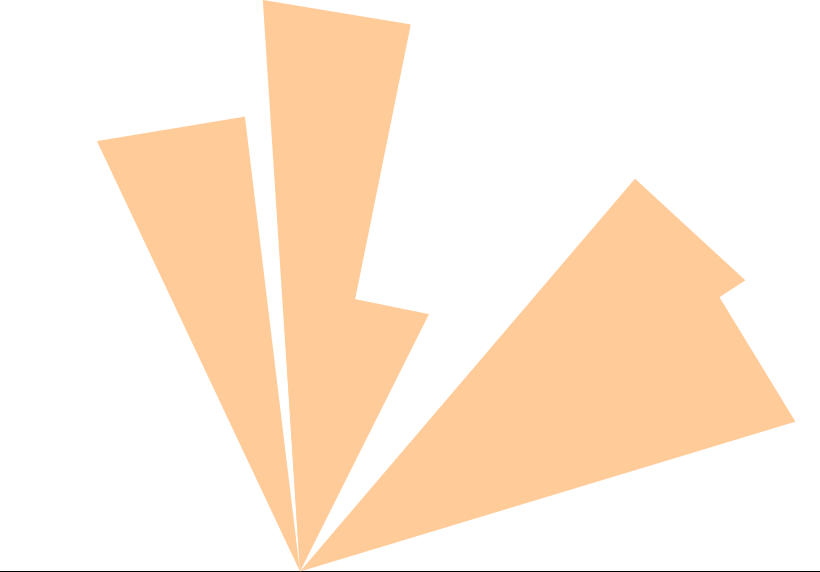
\includegraphics[width=0.6\textwidth]{pics/optimal-tri.png}
  		\captionof{figure}{Optimale Anordnung für eine Summe kleiner $180\degree$}
  	\par}
  \end{kasten} ~\\
 Sollte die Summe jedoch größer sein, ist es nicht mehr so einfach, eine optimale Lösung zu finden. Genauer gesagt kann man ab diesem Punkt nur noch eine Heuristik einsetzen, die ein möglichst gutes Ergebnis liefert. Dabei stellt sich heraus:
 \begin{kasten}
 	Es scheint sinnvoll zu sein, eine Teilmenge der Dreiecke zu finden, für die $\sum \varphi_i < 180\degree$ gilt. Für diese kann die in der vorherigen Beobachtung beschriebene Strategie angewandt werden. \\ \\
 	Nun müssen aber noch die übriggebliebenen Dreiecke angeordnet werden. %TODO wie am besten?
 \end{kasten}
  \subsubsection{Subset Sum und ein DP-Algorithmus}
  Um anhand der Winkel der Dreiecke die jeweils (anfangs z.B. in einem Halbkreis) zu platzierenden Dreiecke zu ermitteln, muss man das Subset-Sum-Problem lösen. Dabei ist eine Menge von ganzen Zahlen $I = \{w_1,...,w_n\} (w_i \in \mathbb{Z})$ gegeben. Nun wird eine Teilmenge $S$ mit maximaler Summe gesucht, die aber nicht größer als eine obere Schranke $c$ (in diesem Fall z.B. $180\degree$ bzw. $\pi$) ist. Formal erfüllt $S$ also folgende Eigenschaften:
  \begin{equation}
  S = \arg \max_{S \in 2^I} \sum_{w_j \in S} w_j
  \end{equation}
  \begin{equation}
  \sum_{w_j \in S} \leq c
  \end{equation}
  Leider ist das Subset-Sum-Problem aber NP-vollständig und somit grundsätzlich nicht effizient lösbar. Ist $c$ jedoch klein genug, existiert ein Dynamic-Programming-Algorithmus zur Lösung des Problems in pseudopolynomieller Zeit.\cite{Src:dpsum} Dazu lässt sich eine DP-Funktion definieren, die mittels einer DP-Tabelle effizient berechnet werden kann:
  \begin{equation}
  dp(i,sum) = 
  \begin{cases}
  false & sum > 0 \wedge i = 0 \\
  true & sum = 0 \\
  dp(i-1,sum) \vee dp(i-1,sum-w_i) & \, \text{sonst}
  \end{cases}
  \end{equation}
  Diese Funktion gibt an, ob sich eine Summe von $sum$ mit den ersten $i$ Elementen der Menge erreichen lässt. Die Funktion baut darauf auf, dass es an jeder Stelle genau zwei Möglichkeiten gibt: Entweder das aktuelle Element wird nicht in das Subset aufgenommen (dann muss man die Summe mit den anderen $i-1$ Elementen erreichen) oder das Element wird in das Subset aufgenommen (dann muss man mit $i-1$ Elementen nur noch eine um $w_i$ verringerte Summe erreichen). \\ \\
  Nun gibt $dp(n,c)$ an, ob es möglich ist, mit allen Elementen die Summe $c$ zu erreichen. Doch da diese Summe oft nicht exakt erreicht werden kann, muss man $c$ entsprechend oft dekrementieren, bis $dp(n,c) = true$ ist und es möglich ist, diese Summe zu erreichen. \\ \\
  Um aus der DP-Tabelle nun das eigentliche Subset zu erhalten, muss man die Lösung backtracen.\cite{Src:dpbacktrace} Dabei betrachtet man für jedes Element $w_i$ einerseits die Möglichkeit, dass das Element enthalten ist, und andererseits, dass das Element nicht enthalten ist. Wenn eine dieser Möglichkeiten laut DP-Tabelle möglich ist, kann man rekursiv eine Lösung für das entsprechende Feld für $i-1$ generieren und dann das aktuelle Element anhängen oder nicht (je nachdem). Am Ende erhält man dann ein mögliches Subset.
  \\ \\
  Da man eine DP-Tabelle mit $n \cdot c$ Elementen ausfüllt, ergibt sich für diesen Algorithmus somit auch eine Laufzeit in $\mathcal{O}(n \cdot c)$, also in pseudopolynomieller Zeit.
  \\ \\
  Mittels dieses Subset-Sum-Algorithmus ist es möglich, Dreiecke so auszuwählen, dass ihre kleinsten Winkel $\varphi_i$ einen gegebenen freien Winkel (z.B. den Halbkreis oberhalb der x-Achse) möglichst gut ausnutzen. Dadurch können die Dreiecke relativ dicht gepackt und der Gesamtabstand verkleinert werden. Entsprechend sind für diese Aufgabe die $w_i = \varphi_i$. \\ \\
   Da es sich bei den Winkeln in der Realität jedoch um Gleitkommazahlen handelt, müssen diese zunächst in Festkommazahlen mit wenigen Nachkommastellen umgewandelt und anschließend mit einem festen Faktor (eine entsprechende Zehnerpotenz) multipliziert werden, damit man natürliche Zahlen erhält, die vom Algorithmus verarbeitet werden können.
  \subsubsection{Der Algorithmus zur Platzierung der Dreiecke}
  \subsubsection{Implementierte Verbesserungen}
  \subsection{Optimalität des Algorithmus und Verbesserungsmöglichkeiten}
 \subsection{Laufzeitbetrachtung und NP-Vollständigkeit}
 %TODO Laufzeit
 Eine Frage, die sich hierbei auch stellt, ist diejenige, ob es für dieses Problem einen in Polynomialzeit terminierenden Algorithmus geben kann, der eine optimale Lösung liefert. Dies entspricht der Frage, ob das Problem in der Klasse $NPC$\footnote{Genaugenommen ist diese Klasse nur für Entscheidungsprobleme definiert, daher handelt es sich bei diesem Suchproblem um NP-Äquivalenz.} (NP-vollständig bzw. NP-complete) liegt. Ich vermute, dass dies der Fall ist, kann es jedoch nicht beweisen. \\ \\
 Zum Beweis, dass ein Problem in $NPC$ liegt, werden zwei Voraussetzungen benötigt:
 \begin{enumerate}
 	\item Eine deterministisch arbeitende Turingmaschine benötigt nur Polynomialzeit, um zu entscheiden, ob eine z.B. von einer Orakel-Turingmaschine vorgeschlagene Lösung tatsächlich eine Lösung des Problems ist. Dies ist hier der Fall, denn wenn eine Lösung vorgeschlagen wird, kann man in Polynomialzeit überprüfen, ob es sich dabei um eine erlaubte Dreiecksanordnung handelt. \\ \\ Dazu überprüft man alle vier Bedingungen dafür. Die ersten beiden Bedingungen lassen sich einfach für jedes Dreieck in konstanter Zeit, insgesamt also in $\mathcal{O}(n)$, überprüfen. Für die dritte Bedingung (Kongruenz) ist dies mithilfe von Kongruenzsätzen ebenfalls in linearer Zeit möglich. Bei der vierte Bedingung  (keine Überlappung) muss man alle Dreieckspaare, insgesamt also $\mathcal{O}(n^2)$, auf Überlappung überprüfen. Insgesamt erhält man mit $\mathcal{O}(n^2)$ also Polynomialzeit.
 	\item Das Problem ist NP-schwer. Das bedeutet, dass alle anderen NP-schweren Probleme auf dieses Problem in Polynomialzeit zurückgeführt werden können. Es ist also eine Polynomialzeitreduktion notwendig. Dabei ist ein Problem aus NPC als Ausgangsproblem nötig, wie z.B. 3-Satisfiability. Eine solche Reduktion zu vollziehen, ist mir jedoch nicht möglich.\footnote{Auch wenn eine Beziehung zwischen \textit{3}-SAT und \textit{Drei}ecken natürlich naheliegt.}
 \end{enumerate}
\begin{thebibliography}{xx}
	\bibitem[1] {Src:dpsum} GeeksforGeeks-Artikel zur DP-Lösung von Subset Sum, \url{https://www.geeksforgeeks.org/subset-sum-problem-dp-25/}
	\bibitem[2]{Src:dpbacktrace} GeeksforGeeks-Artikel zum Backtracen bei der DP-Lösung, \url{https://www.geeksforgeeks.org/perfect-sum-problem-print-subsets-given-sum/}
	\bibitem[3]{Src:pack} Wikipedia-Artikel zu Packproblemen, \url{https://en.wikipedia.org/wiki/Packing_problems}
	\bibitem[4] {Src:dreh} Wikipedia-Artikel zu Drehmatrizen, \url{https://de.wikipedia.org/wiki/Drehmatrix} und Stack-Overflow-Antwort zur Umsetzung in C++, \url{https://stackoverflow.com/questions/2259476/rotating-a-point-about-another-point-2d}
\end{thebibliography}
\section{Umsetzung}
\subsection{Allgemeine Hinweise zur Benutzung}
Das Programm wurde in C++ implementiert und benötigt bis auf die \textit{Standard Library} (STL) und die beigelegte \texttt{argparse}-Library\footnote{\url{https://github.com/hbristow/argparse}},die für die Verarbeitung der Konsolenargumente zuständig ist, keine weiteren Bibliotheken. Es wurde unter Linux kompiliert und getestet; auf anderen Betriebssystemen müsste mit G++ erneut kompiliert werden. \\ \\
Die Eingabe und Ausgabe des Programms erfolgt in Dateien, die mithilfe der Konsolenparameter frei gewählt werden können. Dafür gibt es folgende Parameter:
\begin{verbatim}
Usage: ./main --input INPUT --svg SVG --output OUTPUT
\end{verbatim}
\subsection{Struktur des Programms und Implementierung der Algorithmen}
\subsubsection{Die Datei \texttt{main.cpp}}
\texttt{main.cpp} enthält ausschließlich Funktionen, die für Eingabe und Ausgabe des Programms zuständig sind. Aus diesem Grund wird der Quellcode dieser Datei auch nicht mit abgedruckt.
\subsubsection{Die Datei \texttt{triangles.cpp}}
\subsubsection{Die Datei \texttt{triangleAlgorithm.cpp}}
\section{Beispiele}
\subsection*{Laufzeiten}
\begin{table}[H]
	\begin{tabular}{|c|c|c|} 
		\hline
		Beispiel                                      & Dreiecksanzahl & Laufzeit (ca.)       \\ \hline \hline
		dreiecke1.txt                              & 5     & 8 Millisekunden    \\
		dreiecke2.txt                              & 5      & 8 Millisekunden     \\
		dreiecke3.txt                              & 12      & 11 Millisekunden     \\
		dreiecke4.txt                              & 23      & 10 Millisekunden    \\
		dreiecke5.txt                              & 37      & 27 Millisekunden    \\ \hline
	\end{tabular}
\end{table}
Die Laufzeiten wurden mit dem Linux-Befehl \texttt{time} bestimmt. Dazu wurde ein PC mit einem Intel Core i7 und 8 GB RAM verwendet und das Programm mit der Option \texttt{-O3} kompiliert. Sie sind demzufolge nur grobe Orientierungswerte, die von der verwendeten Hardware abhängen. Es lässt sich aber erkennen, dass der Algorithmus sehr effizient ist und selbst größere Beispiele extrem schnell lösen kann, auch wenn die Ergebnisse nicht immer optimal sind.
\subsection{Beispiel 1}
\begin{figure}[H] 
	\includesvg[width=\textwidth]{../Aufgabe2-Implementierung/examples/out/dreiecke1.svg}
	\caption{Die Dreiecksanordnung für das Beispiel 1}
\end{figure}
\RecustomVerbatimCommand{\VerbatimInput}{VerbatimInput}%
{fontsize=\footnotesize,
	%
	frame=lines,  % top and bottom rule only
	framesep=2em, % separation between frame and text
	rulecolor=\color{Gray},
	%
	label=\fbox{\color{Black} Ausgabe für Beispiel 1},
	labelposition=topline,
	numbers=left,
	%
	commandchars=\|\(\), % escape character and argument delimiters for
	% commands within the verbatim
	commentchar=*        % comment character
}
\VerbatimInput{../Aufgabe2-Implementierung/examples/out/dreiecke1-out.txt}
\subsection{Beispiel 2}
\begin{figure}[H] 
	\includesvg[width=\textwidth]{../Aufgabe2-Implementierung/examples/out/dreiecke2.svg}
	\caption{Die Dreiecksanordnung für das Beispiel 2}
\end{figure}
\RecustomVerbatimCommand{\VerbatimInput}{VerbatimInput}%
{fontsize=\footnotesize,
	%
	frame=lines,  % top and bottom rule only
	framesep=2em, % separation between frame and text
	rulecolor=\color{Gray},
	%
	label=\fbox{\color{Black} Ausgabe für Beispiel 2},
	labelposition=topline,
	numbers=left,
	%
	commandchars=\|\(\), % escape character and argument delimiters for
	% commands within the verbatim
	commentchar=*        % comment character
}
\VerbatimInput{../Aufgabe2-Implementierung/examples/out/dreiecke2-out.txt}
\subsection{Beispiel 3}
\begin{figure}[H] 
	\includesvg[width=\textwidth]{../Aufgabe2-Implementierung/examples/out/dreiecke3.svg}
	\caption{Die Dreiecksanordnung für das Beispiel 3}
\end{figure}
\RecustomVerbatimCommand{\VerbatimInput}{VerbatimInput}%
{fontsize=\footnotesize,
	%
	frame=lines,  % top and bottom rule only
	framesep=2em, % separation between frame and text
	rulecolor=\color{Gray},
	%
	label=\fbox{\color{Black} Ausgabe für Beispiel 3},
	labelposition=topline,
	numbers=left,
	%
	commandchars=\|\(\), % escape character and argument delimiters for
	% commands within the verbatim
	commentchar=*        % comment character
}
\VerbatimInput{../Aufgabe2-Implementierung/examples/out/dreiecke3-out.txt}
\subsection{Beispiel 4}
\begin{figure}[H] 
	\includesvg[width=\textwidth]{../Aufgabe2-Implementierung/examples/out/dreiecke4.svg}
	\caption{Die Dreiecksanordnung für das Beispiel 4}
\end{figure}
\RecustomVerbatimCommand{\VerbatimInput}{VerbatimInput}%
{fontsize=\footnotesize,
	%
	frame=lines,  % top and bottom rule only
	framesep=2em, % separation between frame and text
	rulecolor=\color{Gray},
	%
	label=\fbox{\color{Black} Ausgabe für Beispiel 4},
	labelposition=topline,
	numbers=left,
	%
	commandchars=\|\(\), % escape character and argument delimiters for
	% commands within the verbatim
	commentchar=*        % comment character
}
\VerbatimInput{../Aufgabe2-Implementierung/examples/out/dreiecke4-out.txt}
\subsection{Beispiel 5}
\begin{figure}[H] 
	\includesvg[width=\textwidth]{../Aufgabe2-Implementierung/examples/out/dreiecke5.svg}
	\caption{Die Dreiecksanordnung für das Beispiel 5}
\end{figure}
\RecustomVerbatimCommand{\VerbatimInput}{VerbatimInput}%
{fontsize=\footnotesize,
	%
	frame=lines,  % top and bottom rule only
	framesep=2em, % separation between frame and text
	rulecolor=\color{Gray},
	%
	label=\fbox{\color{Black} Ausgabe für Beispiel 5},
	labelposition=topline,
	numbers=left,
	%
	commandchars=\|\(\), % escape character and argument delimiters for
	% commands within the verbatim
	commentchar=*        % comment character
}
\VerbatimInput{../Aufgabe2-Implementierung/examples/out/dreiecke5-out.txt}
 \section{Quellcode}
 \renewcommand{\listingscaption}{Quellcode}
 
 \begin{longlisting}
 	
 	\cppfile{../Aufgabe2-Implementierung/triangles.cpp}
 	\caption{Die Datei \texttt{triangles.cpp}, die die Klassen \texttt{Triangle}, \texttt{Vektor} und \texttt{Point} und nützliche Hilfsfunktionen für den eigentlichen Algorithmus enthält}
 	
 	\cppfile{../Aufgabe2-Implementierung/triangleAlgorithm.cpp}
 	\caption{Die Datei \texttt{triangleAlgorithm.cpp}, die alle wesentlichen Bestandteile des Algorithmus enthält}
 \end{longlisting}
 
 \end{document}